% Version History
% 2020-10-27  	    Holger Graf
%                   Licence CC BY 4.0
%					Link: https://www.overleaf.com/latex/templates/thesis-template-microeconomics-at-fsu-jena/shqhkgcqtvsn
%					Accessed 18.01.2023
% 2023-02-01		Adapted by Ines Rieger
%					Licence CC BY 4.0
%					Lehrstuhl für Erklärbares Maschinelles Lernen
%					Universität Bamberg
% Please adapt this tex file for your thesis

\documentclass{xai-thesis}

\usepackage{graphicx}
\usepackage{setspace}
\usepackage{hyperref} % use \usepackage[hidelinks]{hyperref} to hide boxes
\usepackage[utf8]{inputenc} % depends on the font encoding that you are using
\usepackage[round]{natbib}
\usepackage{comment}

\input{math_commands.tex}

\begin{document}
% ----------------------------------------------------------------------------
% Details for the titlepage
% ----------------------------------------------------------------------------
\thesisTitle{CNN-based Classification of I-123 ioflupane dopamine transporter 
SPECT brain images to support the diagnosis of Parkinson’s disease with Decision Confidence Estimation}
\thesisType{Master Thesis} % 'Master Thesis' or 'Bachelor Thesis'
\thesisAuthor{Aleksej Kucerenko}
\thesisGrade{Master of Science in Applied Computer Science}
\thesisFirstSupervisor{The name of your first supervisor} % your supervising professor
\thesisSecondSupervisor{The name of your second supervisor, if applicable} % if you are supervised by additional advisors, e.g phd students at the chair or a  supervisor in a company (write company after the name of the supervisor)
\thesisDate{\today}

% Print titlepage
\thesisMakeTitle

% ----------------------------------------------------------------------------
% Abstract
% ----------------------------------------------------------------------------
\clearpage
\pagenumbering{roman}
\pagestyle{plain}

\subsection*{Abstract}
Short summary of your thesis (max. 1 page) \ldots

\clearpage
\subsection*{Abstract}
Kurze Zusammenfassung Ihrer Abschlussarbeit (max. 1 Seite) \ldots

% ----------------------------------------------------------------------------
% Acknowledgements
% ----------------------------------------------------------------------------
\clearpage
\subsection*{Acknowledgements}
If you want to thank anyone (optional) \ldots

% ----------------------------------------------------------------------------
% Table of contents
% ----------------------------------------------------------------------------
\clearpage
%\thispagestyle{empty}
\tableofcontents

% ----------------------------------------------------------------------------
% List of figures/tables/acronyms
% ----------------------------------------------------------------------------
\clearpage
\phantomsection
\addcontentsline{toc}{section}{List of Figures}
\listoffigures
% --------------------------
\clearpage
\phantomsection
\addcontentsline{toc}{section}{List of Tables}
\listoftables
% --------------------------
\clearpage
\phantomsection
\addcontentsline{toc}{section}{List of Acronyms}
\section*{List of Acronyms}
\begin{tabular}{@{}ll}
AI & Artificial Intelligence\\
\end{tabular}

% ----------------------------------------------------------------------------
% Notation
% ----------------------------------------------------------------------------
\clearpage
\section*{Notation}
\input{math_notation.tex}

% --------------------------

% ----------------------------------------------------------------------------
% Contents
% ----------------------------------------------------------------------------
\cleardoublepage
\pagestyle{headings}
\pagenumbering{arabic}
\setcounter{page}{1}

% Hint: It is advisable to split the thesis into several tex files organized by sections. You can use thesis.tex as the main file and include any other tex file with \input(introduction.tex)

\section{Introduction}
\label{sec:intro}

% Parkinson's disease (intro)

Parkinson's disease (PD) is the second most common neurodegenerative disease after Alzheimer's disease [1]. 
It is expected to impose an increasing social and economic burden on societies as populations age [2]. 
The prevalence of PD in industrialized countries is about 1\% in people over 60 years of age [2]. 
The standardized incidence rate of PD is estimated to range between about 10 and about 20 per 100,000 person-years [2]. 
Thus, there are up to 100,000 new PD cases per year in the EU and up to 50,000 in the US.

% PD symptoms and diagnosis
PD is characterized by bradykinesia and variable expression of cardinal symptoms: resting tremor, rigidity, and postural instability [3, 4]. 
However, this combination of symptoms, often referred to as `parkinsonism' or `parkinsonian syndrome' (PS), 
occurs not only in PD (and some rare `atypical' neurodegenerative PS such as multiple system atrophy, progressive 
supranuclear palsy and corticobasal degeneration). 
It also occurs in so-called `secondary' (non-neurodegenerative) PS that can be induced by drugs, head trauma, 
inflammatory or metabolic disorder, as well as other diseases such as essential tremor, dystonic tremor, or normal pressure hydrocephalus [3, 5]. 
A particularly frequent cause of secondary PS is cerebrovascular disease [6]. 
The differentiation between PD and secondary PS is highly relevant, 
because secondary PS might be treated more effectively than PD and some secondary PS may be fully cured.
Yet, the clinical, that is, symptom-based differentiation between PD and secondary PS is challenging in a significant fraction of patients, 
particularly at early disease stages with mild symptoms and in patients with atypical presentation [7, 8]. 
These cases are often referred to as `clinical uncertain parkinsonian syndromes' (CUPS) [9].

% PD medical background
PD, as well as the `atypical' neurodegenerative PS, is associated with progressive loss of substantia nigra pars compacta (SNpc) dopaminergic neurons 
projecting to the striatum [10]. 
Reduced availability of dopamine transporters (DAT) in the striatum is well-validated as a biomarker for 
nigrostriatal degeneration in PD [11-13]. 
It can be detected by single photon emission computed tomography (SPECT) with dopamine transporter (DAT) ligands [14, 15]. 
Reduction of striatal DAT availability is strongly advanced already at the earliest symptomatic (motor) stages of PD, 
because the degeneration of dopaminergic nerve endings in the striatum is an early step in the pathological PD cascade [11-13]. 
Compensatory downregulation of the DAT expression in the remaining nerve endings results in even more pronounced striatal DAT loss [16-18]. 
Secondary PS are as a rule not associated with nigrostriatal degeneration and loss of striatal DAT. 
To differentiate PD from secondary PS based on striatal DAT availability, the radioactively labeled DAT ligand [123I]FP-CIT 
(trade name: $\text{DaTscan}^{\copyright}$) has been licensed as SPECT tracer in both, the US and Europe [19].

% DAT-SPECT method 
A recent review, including a non-systematic meta-analysis, of DAT-SPECT with [$^{123}$I]FP-CIT in PS confirmed high sensitivity (median 93\%) 
and high specificity (median 89\%) of DAT-SPECT for the differentiation of PD from secondary PS in patients with CUPS [20]. 
The review further revealed that DAT-SPECT leads to a change of diagnosis in about 40\% and to a change of treatment in about the same proportion of 
patients with CUPS [20]. 
Thus, DAT-SPECT with [$^{123}$I]FP-CIT is highly diagnostically accurate and has a relevant impact on the diagnosis and treatment of CUPS patients. 
Guidelines from professional neurological societies therefore strongly strengthened the role of DAT-SPECT with [$^{123}$I]FP-CIT in the last years [21]. 
For example, the current version of the S3 guideline “Idiopathic Parkinson syndrome” of the German Society of Neurology states that DAT-SPECT 
\textit{should} be performed at an early disease stage in CUPS. 

% Early detection of PD is desirable
In line with its high accuracy, its relevant impact on patient management, and the strong guideline recommendations, 
DAT-SPECT with [123I]FP-CIT is the most frequent nuclear medicine brain imaging procedure. 
In Europe about 70,000 patients are referred to DAT-SPECT per year, in Germany alone about 10,000, at UKE currently about 400 per year [22]. 
The demographical change in industrial countries is expected to result in a further increase in the number of DAT-SPECT examinations, 
because age is the major risk factor for PD [23]. 
Furthermore, there are early signs of PD such as smell loss and \textit{idiophatic} rapid eye movement sleep and behavioral disorder 
that can precede movement problems by several years, but are not particularly specific for PD [24-26]. 
It becomes increasingly important to detect PD at these early pre-motor stages, because the earlier the treatment is initiated the better 
the chances of moderating the course of PD with disease-modifying drugs[27].

% Automatic and accurate classification of DAT-SPECT desirable
In clinical practice, the interpretation of DAT-SPECT is binary, that is, the nuclear medicine physician has to decide whether the SPECT images 
indicate degeneration of the dopaminergic neurotransmitter system (-> Parkinson's disease) or not (-> secondary PS). 
This decision can be challenging by visual inspection of the tomographic SPECT images, particularly for less experienced readers [28]. 
Thus, DAT-SPECT would benefit from methods for the automatic classification of the images that achieve similar (or better) performance as experienced readers. 
Convolutional neural networks (CNNs) appear particularly promising for this purpose [29-47].

% Difficulty of classification of borderline cases
Yet, there are also `true' borderline cases that cannot be classified with high certainty even by expert readers. 
In DAT-SPECT of CUPS, the proportion of visually inconclusive borderline cases ranges between 5 and 10\% [48, 49]. 
Automatic binary classification of these cases by a CNN might pretend a certainty of the diagnosis that is not actually given. 
It is important, therefore, to identify these cases in order to make sure that the user visually inspects these SPECT images 
in order to check the automatic categorization particulary carefully. 
The user will accept the CNN's decision in some case, overrule the CNN in other cases, and will categorize the remaining cases as 
actually inconclusive (and might recommend follow-up DAT-SPECT after 6-12 months [50]). 

% Sigmoid output alone not suitable for identification of borderline cases
The most obvious approach to identify borderline cases in CNN-based classification would be based on the distance of the CNN's sigmoid output from a predefined decision threshold (e.g., 0.5). 
However, empirically, sigmoid outputs of CNN for classification of DAT-SPECT tend to cluster at the extreme values so that their utility for the identification of borderline cases seems limited.  
As a consequence, this approach is not recommended among practitioners, as it tends to overestimate the certainty of CNN-based classification [51-53].

% Aim of work and overview on the approach

Against this background, the current work aimed to propose and validate a CNN-based approach for the automatic classification of DAT-SPECT 
that allows reliable identification of inconclusive cases that might be misclassified by the CNN when the decision threshold is strictly applied.
The `decision confidence' of the classifier is evaluated on a metric, proposed in the following, that aims to maximize the performance of the classifier
on between-reader consensus cases while minimizing the potential effort of manual inspection originating from inconclusive cases.

Starting from the assumption that between-readers discrepancy in the binary visual interpretation of DAT-SPECT is much more likely in inconclusive cases 
than in conclusive cases, a standard CNN structure was trained for automatic classification of DAT-SPECT using a large training dataset in which each 
SPECT image had been visually classified by three independent readers. 
During the model training phase, the standard-of-truth label was selected randomly from the three independent available reads. 
This way, the same inconclusive image could be presented to the network with different standard-of-truth labels. 
The rationale was that this could allow the network to learn about the uncertainty of these cases, 
and that this would result in sigmoid outputs close to the decision threshold.

This “random label” training (RLT) approach was compared with the conventional majority vote training (MVT) approach. 
In the latter,  the majority vote across the three readers was consistently used as standard-of-truth during the training phase. 
The MVT obviously “hides” the uncertainty associated with between-readers discrepancy from the network. 

To be able to better assess the performance of the CNN-based approaches, univariate and multivariate conventional methods were employed as 
benchmark methods. In addition, the performance of the approaches is also evaluated on independent external datasets.

% Hypotheses

% 1st hypothesis
The primary hypothesis put to test in this work was that the sigmoid output of the CNN is more appropriate for the identification of inconclusive cases 
(by an `inconclusive' range around the decision threshold) when the network is trained with the RLT approach compared to MVT.

To test this hypothesis, the proportion of inconclusive cases required to achieve a given balanced accuracy in the conclusive cases 
was proposed and used as a performance metric.
More precisely, the area under the curve (AUC) of balanced accuracy in conclusive cases versus the proportion of inconclusive cases 
(observed in the test set) was used as a model-agnostic quality metric. 
The AUC does not depend on a specific working point (target balanced accuracy).  
The rationale for this performance metric is that more inconclusive cases would require more attention and manual inspection 
by the attending physician which is considered `expensive'
(“90\% inconclusive cases to achieve the required accuracy in the remaining 10\% of cases is clearly useless”).
Therefore the utility of the classifier for widespread use in clinical practice depends on its `decision confidence', 
e.g. the proportion of inconclusive cases to be accepted to achieve a predefined balanced accuracy in the remaining conclusive cases. 

% 2nd hypothesis
The following secondary hypotheses were put to test. First, CNN-based classification outperforms conventional methods in terms of balanced accuracy, 
both univariate and multivariate conventional methods. 
The specific binding ratio (SBR) of the tracer uptake in the putamen was used for the univariate analyses. 
Current procedure guidelines recommend the putaminal SBR to support the visual interpretation of DAT-SPECT in everyday clinical patient care [54]. 
The putaminal SBR characterizes the contrast of the tracer uptake (= intensity) in the putamen relative to the mean tracer uptake in a reference 
region void of DAT [55]. 
The putaminal SBR is assumed to be proportional to the density of DAT in the putamen [55]. 
As a multivariate benchmark method, a random forest approach was implemented using the expression profile of a set of covariance patterns as input. 
The covariance patterns were identified by principal component analysis in the training dataset. 

% 3rd hypothesis
Second, CNN-based classification demonstrates enhanced generalizability, such as being more robust regarding varying image characteristics 
(e.g., spatial resolution) 
associated with the use of different acquisition hardware 
(different SPECT cameras, different collimators\dots) 
and different reconstruction and correction methods (application of resolution recovery, application of attenuation correction\dots). 
To test this hypothesis, the classification methods were compared in two test datasets fully independent of the training dataset.

% Summary of research questions
The following research questions are addressed: 
\begin{itemize}
    \item When comparing the CNN-based approaches, how does the RLT approach perform compared to the MVT approach? 
    Is the performance metric proposed in this work practically suitable for the comparison of different approaches?

    \item How do the CNN-based approaches perform on diverse testing data compared to conventional approaches?
    What conclusions can be made regarding the generalizability of the approaches under test?
    
\end{itemize}


% thesis structure




\section{Background}
\label{sec:background}

\subsection{DAT-SPECT for Detecting Parkinson's Disease}
\label{subsec:datspect}

% DAT-SPECT - Medical background

Parkinson's disease (PD) and 'atypical' neurodegenerative Parkinsonian syndromes (PS) 
are both associated with the progressive loss of dopaminergic neurons in the substantia nigra pars compacta (SNpc) 
that project to the striatum~\citep{Piggott1999}.
The reduced availability of dopamine transporters (DAT) in the striatum is a well-validated biomarker 
for nigrostriatal degeneration in PD~\citep{Bernheimer1973, Fazio2018, Niznik1991}.
It can be detected by single photon emission computed tomography (SPECT) 
with dopamine transporter (DAT) ligands~\citep{Kuikka1995, Abi-Dargham1996}.
The reduction in striatal DAT availability is significantly advanced 
even in the earliest symptomatic (motor) stages of PD, 
as the degeneration of dopaminergic nerve endings in the striatum represents 
an early step in the pathological PD cascade~\citep{Bernheimer1973, Fazio2018, Niznik1991}.
The compensatory downregulation of the DAT expression in the remaining nerve endings 
leads to a more pronounced loss of striatal DAT~\citep{Lee2000, Saari2017, Honkanen2019}.
Secondary PS's are typically not associated with nigrostriatal degeneration or the loss of striatal DAT. 
To differentiate PD from secondary PS based on striatal DAT availability, 
the radiolabeled DAT ligand [$^{123}$I]FP-CIT (trade name: $\text{DaTscan}^{\copyright}$) 
has been approved as a SPECT tracer in both the US and Europe~\citep{Neumeyer1994}.

% DAT-SPECT for differentiation of PD from PS's

A recent review, which involved a non-systematic meta-analysis of DAT-SPECT with [$^{123}$I]FP-CIT in patients with PS, 
confirmed that DAT-SPECT exhibits high sensitivity (median 93\%) and high specificity (median 89\%) 
in differentiating PD from secondary PS in patients with 
clinically uncertain parkinsonian syndrome (CUPS)~\citep{Buchert2019-ya}.
Moreover, the review demonstrated that DAT-SPECT results in a change in diagnosis for about 40\% of patients with CUPS
and leads to a change in treatment for a similar proportion of these patients~\citep{Buchert2019-ya}. 
Thus, DAT-SPECT with [$^{123}$I]FP-CIT is a highly accurate diagnostic method
that significantly influences the diagnosis and treatment of patients with CUPS.
Guidelines from professional neurological societies have therefore strongly emphasized 
the role of DAT-SPECT with [$^{123}$I]FP-CIT in recent years~\citep{Tatsch2013}.
For example, the current version of the S3 guideline “Idiopathic Parkinson syndrome” of the 
German Society of Neurology states that DAT-SPECT \textit{should} be conducted at an early disease stage in CUPS patients.

\subsection{Convolutional Neural Networks for Image Classification}
\label{subsec:randfors}

% CNN

% Random forest 



\section{Methods}
\label{sec:methods}

\subsection{Software Tools and Libraries}
\label{subsec:libs}

//TODO

\subsection{Development Data Preparation}

In the following, the data preparation techniques applied to the development dataset are explained in detail.

\subsubsection{Data Preprocessing}
\label{subsubsec:img_preprocess_dev}

% Preprocessing of development dataset

% TODO -> wo "as described previously" -> näher beschreiben

Individual DAT-SPECT images were stereotactically normalized to the anatomical space of the Montreal Neurological Institute (MNI) 
using the Normalize tool of the Statistical Parametric Mapping software package (version SPM12) and a set of custom DAT-SPECT templates 
representative of normal and different levels of Parkinson-typical reduction of striatal uptake as target [73]. 
The voxel size of the stereotactically normalized images was 2x2x2 mm$^{3}$. 
Intensity normalization was achieved by voxelwise scaling to the individual 75th percentile of the voxel intensity in a reference region 
comprising the whole brain without striata, thalamus, brainstem, cerebellum, and ventricles [74]. 
The resulting images are distribution volume (DVR) images. 
A 2-dimensional transversal DVR slab of 12mm thickness and 91x109 pixels with 2 mm edge length was obtained by averaging 6 transversal slices through the striatum [75]. 

\subsubsection{Data Augmentation}
\label{subsec:augment}

Data augmentation was applied to the development dataset to increase the heterogeneity of the data.
To enhance robustness across various attenuation correction and scatter correction methods, 
each image was generated in a version with and without attenuation and scatter corrections applied.
Also 3D-smoothing was employed for augmentation using an isotropic Gaussian kernel with various 
Full Width at Half Maximum (FWHM) values (FWHM = 10, 12, 14, 16, 18mm).
Thereby an augmented dataset of 20,880 images in total was constructed based on 1,740 cases.
An example of two cases augmented using the described techniques is depicted in Figure~\ref{fig:dev_dataset}.

\begin{figure}[t]
    \centering
    \colorbox{black}{%
     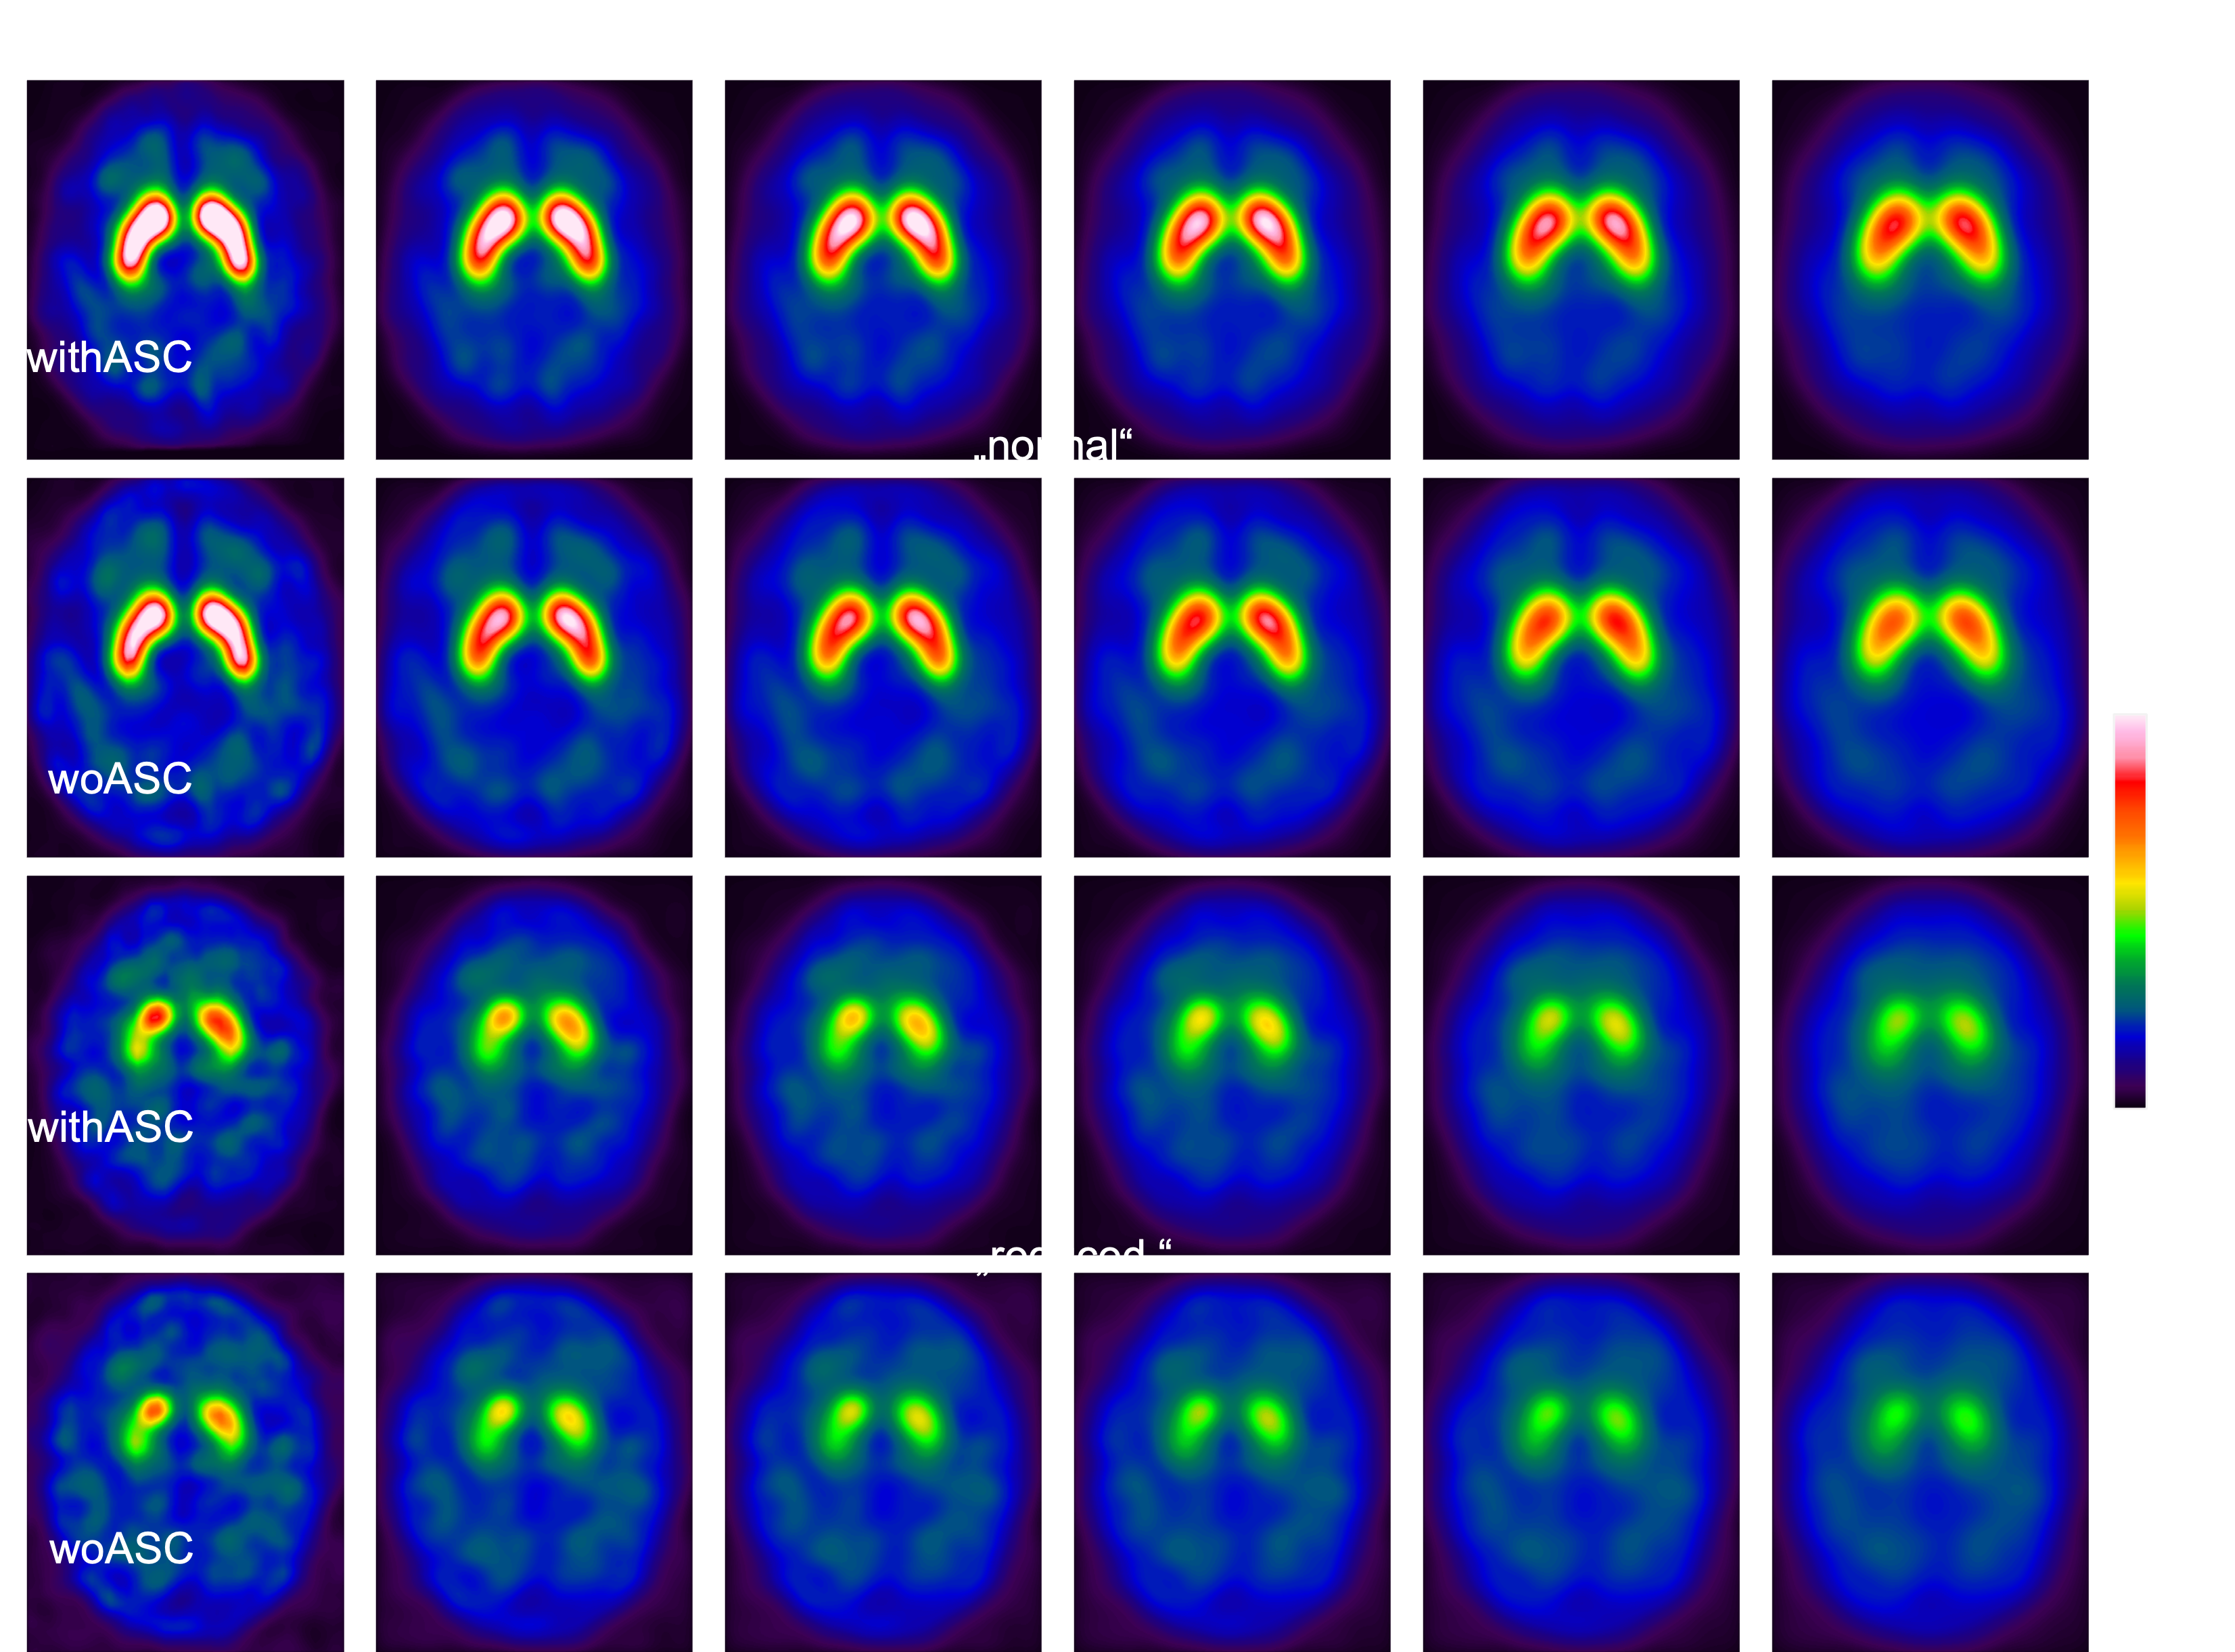
\includegraphics[width=0.9\textwidth]{content/figures/dev_dataset.png}%
     }
    \caption{Images obtained through augmentation of two sample cases from the development dataset, 
    a healthy case (above) and a PD case with reduced availability of DAT in the striatum (below).} 
    \label{fig:dev_dataset}
  \end{figure} 

\subsubsection{Dataset Splitting}
\label{subsec:split}

% How was dev dataset split
The augmented development dataset was split into three subsets: train set (60\%), validation set (20\%) 
and test set (20\%).
While splitting the data it was ensured that the augmented images belonging to a concrete patient were put 
only into one subset.
Thereby inter-subset data leakage was prohibited.
Ten different random splits were created to train and test each of the methods.

\subsection{Univariate benchmark: Specific Binding Ratio}
\label{subsec:sbr}

% TODO -> wo "as described previously" -> näher beschreiben

The unilateral [$^{123}$I]FP-CIT specific binding ratio (SBR) was used as a benchmark classification method.
Here, the SBR in left and right putamen was obtained by hottest voxels (HV) analysis of the stereotactically normalized 
DVR image using large unilateral putamen masks predefined in MNI space [46].
It can be calculated as 

\begin{equation}\label{eq:sbr}
  \text{HV-SBR}_{unilateral} = \frac{1}{K} \sum_{k} \hat{I}_{k, ROI} \;,
\end{equation}

where $\hat{I}_{k, ROI}$ are the \textit{normalized} voxel intensities of the $K$-hottest voxels of the unilateral ROI.
The voxel intensities of the hottest voxels are normalized to the 75th percentile of the voxel intensities 
in the reference region associated with non-specific binding [46].
The minimum of the HV-SBR values from the left and right hemispheres was used for the analysis.
An in-depth elaboration on SBR analysis can be found in [46].

The SBR-based classifier was obtained as follows.
First the SBR was calculated for each case in the training set.
Then the optimal cutoff on the SBR was determined using ROC analysis and the Youden criterion~\citep{Youden1950}.
The determined optimal cutoff was then used as the decision boundary between normal cases (NC) and Parkinson's disease (PD) 
and evaluated on the test split of the development dataset for each of the 10 random splits.
Also the determined cutoff was evaluated on the PPMI and MPH datasets described in Section~\ref{subsec:external_dataset}.

\subsection{Multivariate benchmark: PCA-enhanced Random Forest}
\label{subsec:pca_rfc}

As a further benchmark, a random forest classifier was trained on PCA-transformed features of the training set.
Therefore first a PCA model with 10 principle components was initialized and fit to the training set features to obtain 
the principle components of the training set.
Then the principle components were used to transform the training set to the lower-dimensional space.
An example of the principle components of the training set for one of the random splits is depicted in Figure~\ref{fig:pca_components}.

The training data transformed by the principle components is then used to train a random forest classifier with 100 decision trees.
As hyperparameters, the Gini impurity was used to assess split quality, 
with a minimum of 2 samples required to split an internal node and 1 sample needed at a leaf node.
The trained random forest classifier was evaluated on the test split of the development dataset for each of the 10 random splits.
In addition the trained model was tested on the PPMI and MPH datasets described in Section~\ref{subsec:external_dataset}.

\begin{figure}[ht]
  \centering
  \includegraphics[width=1.0\textwidth]{content/figures/pca_components_splittrain.png}
  \caption{Principle components of the training set (development dataset) for one of the random splits.} 
  \label{fig:pca_components}
\end{figure} 

\subsection{CNN-based classification - MVT and RLT}
\label{subsec:cnn_based_classification_mvt_rlt}



\subsection{CNN-based classification - Regression}
\label{subsec:cnn_based_classification_regression}



\subsection{Determination of Inconclusive Ranges on the Probabilistic Output}
\label{subsec:determinationInconcl}


// TODO

On the validation set...

Determination of inconclusive ranges given a set of target percentages of inconclusive cases (0.2\% to 20.0\%, step 0.2\%).

e.g. what is the inconclusive range corresponding to 10\% of test cases being classified as inconclusive?

The determined inconclusive ranges were then used to compute the balanced accuracy on the conclusive cases.


\input{content/4_evaluation.tex}

\input{content/5_discussion.tex}

\input{content/6_conclusion.tex}

% --------------------------
\clearpage
\begin{appendix}
	\section{Appendix}
	If needed for supplementary material, such as detailed description of data collection, tables, or figures.
	
\end{appendix}

% ----------------------------------------------------------------------------
% Bibliography
% ----------------------------------------------------------------------------
\clearpage
\renewcommand\refname{Bibliography}
\addcontentsline{toc}{section}{Bibliography}
\bibliography{bibliography}
\bibliographystyle{plainnat}

% ----------------------------------------------------------------------------
% Statutory declaration
% ----------------------------------------------------------------------------
\clearpage
\makeThesisDeclaration

\end{document}

